\documentclass[a4paper]{article}
\setlength{\columnsep}{40pt}
\usepackage{graphicx} 
\usepackage[a4paper,margin=0.5in]{geometry}
\usepackage{amsmath}
\usepackage{booktabs}
\usepackage{float}
\usepackage{hyperref}

\title{Bobcats, Coyotes \& Foxes}
\author{Salvin Chowdhury}
\date{\today}

\begin{document}

\setlength{\intextsep}{0pt} 
\setlength{\textfloatsep}{5pt} 

\maketitle
\tableofcontents
\newpage

\section{Introduction}
This paper is for a midterm project dedicated towards replicating the results from a paper on a morphometric modeling approach to distinguishing among
bobcat, coyote, and gray fox scats. This midterm project requires determining the best approach for addressing research questions as shown in Section 1.2. \\

\noindent Understanding the distribution and behavior of various species is fundamental to ecology, as it helps ecologists understand the relationship between
organsims and their environments. There is a lot ecological signifigance behind tracking such species, as researchers can see precisely when individual 
animals depart from one location and arrive at another. Such insights reveal a individual animal's seasonal movements, feeding locations and more. Such
information is valuable because the more ecologists know about animals' seasonal usage of habitats, the more they can protect the areas the animals need to
survive. \\

\noindent Given that adult Gray Foxes have a greater average body length than adult Bobcats, and a smaller average body length than adult Coyotes, we hypothesize 
that Gray Fox scat will exhibit a significantly larger average diameter than Bobcat scat, but a smaller average diameter than Coyote scat.

\subsection{Background Information}
Conservation exologists monitor species populations to assess the health of the ecosystem and just how effective conservation strategies are. While there are
several methods for estimating population sizes, such as mark-recapture and camera-trap surveys, an alternative approach to this is analyzing biological 
remnants such as scat, as performed by Dr. Reid. \\

\noindent In a 2015 study by Dr. Rachel Reid, Reid had investigated whether morphological, biogeochemical and contextual traits distinguish between bobcat, coyote and
fox scat. Morphological traits are the most cost-effective for field identification, while biogeochemical traits require laboratory analysis. 

\subsection{The Research Questions}
The purpose of this paper is to analyze the data to evaluate whether specific morphological or biogeochemical traits can reliably differentiate species. We 
also research biological and ecological factors that explain the observed patterns. The research questions are listed as follows:
\begin{itemize}
    \item Which (if any) morphological and biogeochemical traits distinguish between originating species of the scat samples?
    \item Why do you think those traits differ across species?
\end{itemize}

\subsection{The Diet, Habitat \& Physical Characteristics of Bobcats}
Bobcats are mostly carnivoruous. Their diet consists of a variety of animals, such as rabbits, rodents, wood rats birds, insects and many more. They also
will consume plant material such as grass. Bobcats will also hunt pets or small livestock such as chicken if they're not kept in a secure enclosure. Bobcats
can be found in diverse habitats throughout California. Suitable Bobcat habitat includes vegetation types, brushy stages of low and mid-elevation conifer, 
forests and desert environments. Interestingly, Bobcats prefer areas with dense bush cover. When it comes to physical characteristics, Bobcats are 
medium-sized cats with muscular bodies. They weight between 12 and 25 pounds. Bobcats have a round face with ruffs of fur on the side of the head. They have
pointed ears, and appear to be approximately one quarter of the size of a mountain lion.

\subsection{The Diet, Habitat \& Physical Characteristics of Coyotes}
The diet of a coyote consists mainly only mice, rats, ground squirrels, gophers, rabbits and carrion. They also eat insects and birds. In rural areas of
California, they prey heavily on sheep, cattle and poultry. In urban and suburban areas, domestic cats, dogs and other pets can be food items. Coyotes can
be found in the hotter drier regions of California. They can also be found in mountainous or humid areas in the state. Some physical characteristics of the 
coyote are that they are medium sized animals that belong to the Dog family. They can weigh between 22 to 25 pounds on average, with males being the larger
sex. They also have large erect ears, slender muzzle and a bushy tail. Lastly, they have a distinctive voice and are proficient predators.

\subsection{The Diet, Habitat \& Physical Characteristics of Gray Foxes}
The diet of a gray fox consists mainly of small rodents, birds and berries. They will also eat insects, eggs, acorns and fungi. Gray foxes can be found in
populating coastal or mountain forests at lower elevations. They rarely dig their own dens, but will instead rest in crevices, under boulders and in hollow
logs. Some physical characteristics of Gray Foxes are that it has short legs, a silvery-gray coat with patches of yellow, brown, rust, or white on the 
throat and the belly. Black tipped guard hairs form a dark line down its back to the tip of the tail.

\newpage

\subsection{Population Estimation Methods for Conservation}
Next, we look at the different population estimation methods for conservation. We also look at their strengths and weaknesses. 

\subsubsection{Mark \& Recapture Benefits and Drawbacks}
For mobile organsisms, we use a method called Mark \& Recapture. This method involves marking a sample of captured animals and then releasing them back into 
the environment to allow them to mix with the rest of the population. A common issue with mark-recapture methods is that the process of capturing and marking
the animals changes their behavior. This is otherwise known as a trap response.

\subsubsection{Qudrants Benefits and Drawbacks}
A quadrant is a frame used in ecology to isolate a standard unit of area for the study of the distribution of an item over a large area. Quadrats typically 
occupy an area of 0.25 $m^2$, and are traditionally square. Some benefits it is quick, inexpensive and portable. Some of the disadvantages are it is not 
very accurate and the sample can seem unintentionally biased.

\subsubsection{Transects Benefits and Drawbacks}
A transect is a straight line that cuts through a natural landscape so that standardized observations and measurements can be made. Some advantages of using
transects are it is quick, inexpensive and portable. A disadvantage of transects is that it is often used in inapproriate situations, so care must be taken 
when deciding whether or not to use a transect.

\subsection{Dataset Description}
With regards to the dataset used for perfoming data pre-processing, statistical and visualization techniques, it consists of 110 observations and 19 features.
The features are of two different data types, such as \texttt{categorical}, \texttt{int64} and \texttt{float64}. This is a small dataset, and some of the 
features have null values, which are \texttt{scat\_taper\_mm}, \texttt{scat\_taper\_index}, \texttt{scat\_mass\_grams}, \texttt{d13C}, \texttt{d15N} and 
\texttt{CN Ratio}.

\newpage

\section{Methods}
In this section, we discuss how we cleaned the dataset, including handling of missing values, data type conversions, and any transformations that we applied.
We will also justify any decisions made about outlier treatment (removal, transformation or retention). Moreover, we look at the different statistical and
visualization techniques we've used in this paper and why such approaches were appropriate.

\subsection{Data Type Conversion}
Looking at the dataset, we needed to understand what the features were about. We needed to know what the units were, what the features mean, as well as the 
description of the features. We renamed the columns to indicate some clarity as to what the feature was about, and we also renamed some numerical features
to indicate what the unit of that feature was. After using \texttt{.info()} to look at the data type of each feature, we could see that some of the features
were incorrectly represented as \texttt{int64} or \texttt{object}. For features that have binary values, or features that were missrepresented as 
\texttt{object} we converted them into \texttt{category} using \texttt{.astype()}.

\subsection{Imputing or Dropping?}
When we looked at the size of the dataset, we saw that it was 19 features in total and about 110 observations. In the context of machine learning 
applications, such a dataset is too small to drop any observations that have any missing values. Instead, we chose to impute. When it came to performing
imputations, we needed to decide between the mean and median method if imputation for feature. The reasoning behind each method of imputation is as follows:

\begin{itemize}
    \item \textbf{Mean:} we use the mean for numerical features that are normally distributed
    \item \textbf{Median:} we use the median for numerical features that are skewed and contain outliers
\end{itemize}

\noindent In order to figure out whether a feature is normally distributed or skewed, we need to use data visualization. For situation, we can plot a kernel
density estimation plot for each of the features as well as box plot.

\subsection{Visualization Tehcniques}
When it came to performing visualization techniques, we had to set a response variable, which was \texttt{scat\_species}. Given that the response variable
was categorical, this means we performed our visualizations according to the following rules:

\begin{itemize}
    \item \textbf{Categorical vs Numerical:} for plotting a categorical feature against numerical features, we explored using either box plots or violin plots
    \item \textbf{Categorical vs Categorical:} for plotting a categorical feature against categorical features, we explored using heat maps
\end{itemize}

\noindent The visualizations were performed as we compared the response variable against features from both morphological and biogeochemical traits.

\subsection{Statistical Testing Tehcniques}
When it came to performing statistical testing, we used our previously set response variable which was categorical against a number of categorical and
numerical features, this means we performing our statistical testing according to the following rules:

\begin{itemize}
    \item \textbf{Kruskal-Wallis:} for comparing a categorical variable with multiple values against a numerical variable, it answers the question of whether
    atleast one group defined by the categorical variable differs from at-least one other.
    \item \textbf{$\chi^2$ Test of Independence:} it is a hypothesis test for comparing two categorical variables and measures whether there is a 'dependence' 
    between them
    \item \textbf{Dunn Testing:} used as a post-hoc analysis after a Kruskal-Wallis test to identify which specific groups are significantly different from
    each other.
\end{itemize}

\noindent The statistical tests were performed as we compared the response variables against features from both morphological and biogeochemical traits. The 
justification for all statistical tests and visualizations were all dependent on the type of variable we were dealing against the response variable, and this
will be explained in further detail in Section 3.

\subsection{Family-Wise Error Rate}
When it came to determining the family-wise error rate method for each of the tests, we decided to go with bonferroni correction. It is a multiple comparision
adjustment method that reduces the signifigance level to control for false positives when performing multiple hypothesis tests. The justification behind using
it is that we would like to reduce the likelihood of false positives when performing multiple comparisions. 


\newpage

\section{Results}
In this section, we disucss the different visualization techniques and statistical testing methods that were performed to evaluate the relationships between
the morphological and biogeochemical traits and species. We also determine which traits can be used to distinguish atleast one species from the rest.

\subsection{Histograms \& Boxplots}
In this page, we display all the histograms and box plots of all features that have missing values so that we can justify the method of imputation. 
\vspace{0.5cm}

\begin{figure}[h]
    \centering
    \begin{minipage}{0.63\textwidth}
        \centering
        \includegraphics[width=\linewidth]{C:/GitHub/BobcatsCoyotesFoxes/plots/kde_missing.png}
    \end{minipage}
    \vspace{0.5cm}
    \begin{minipage}{0.63\textwidth}
        \centering
        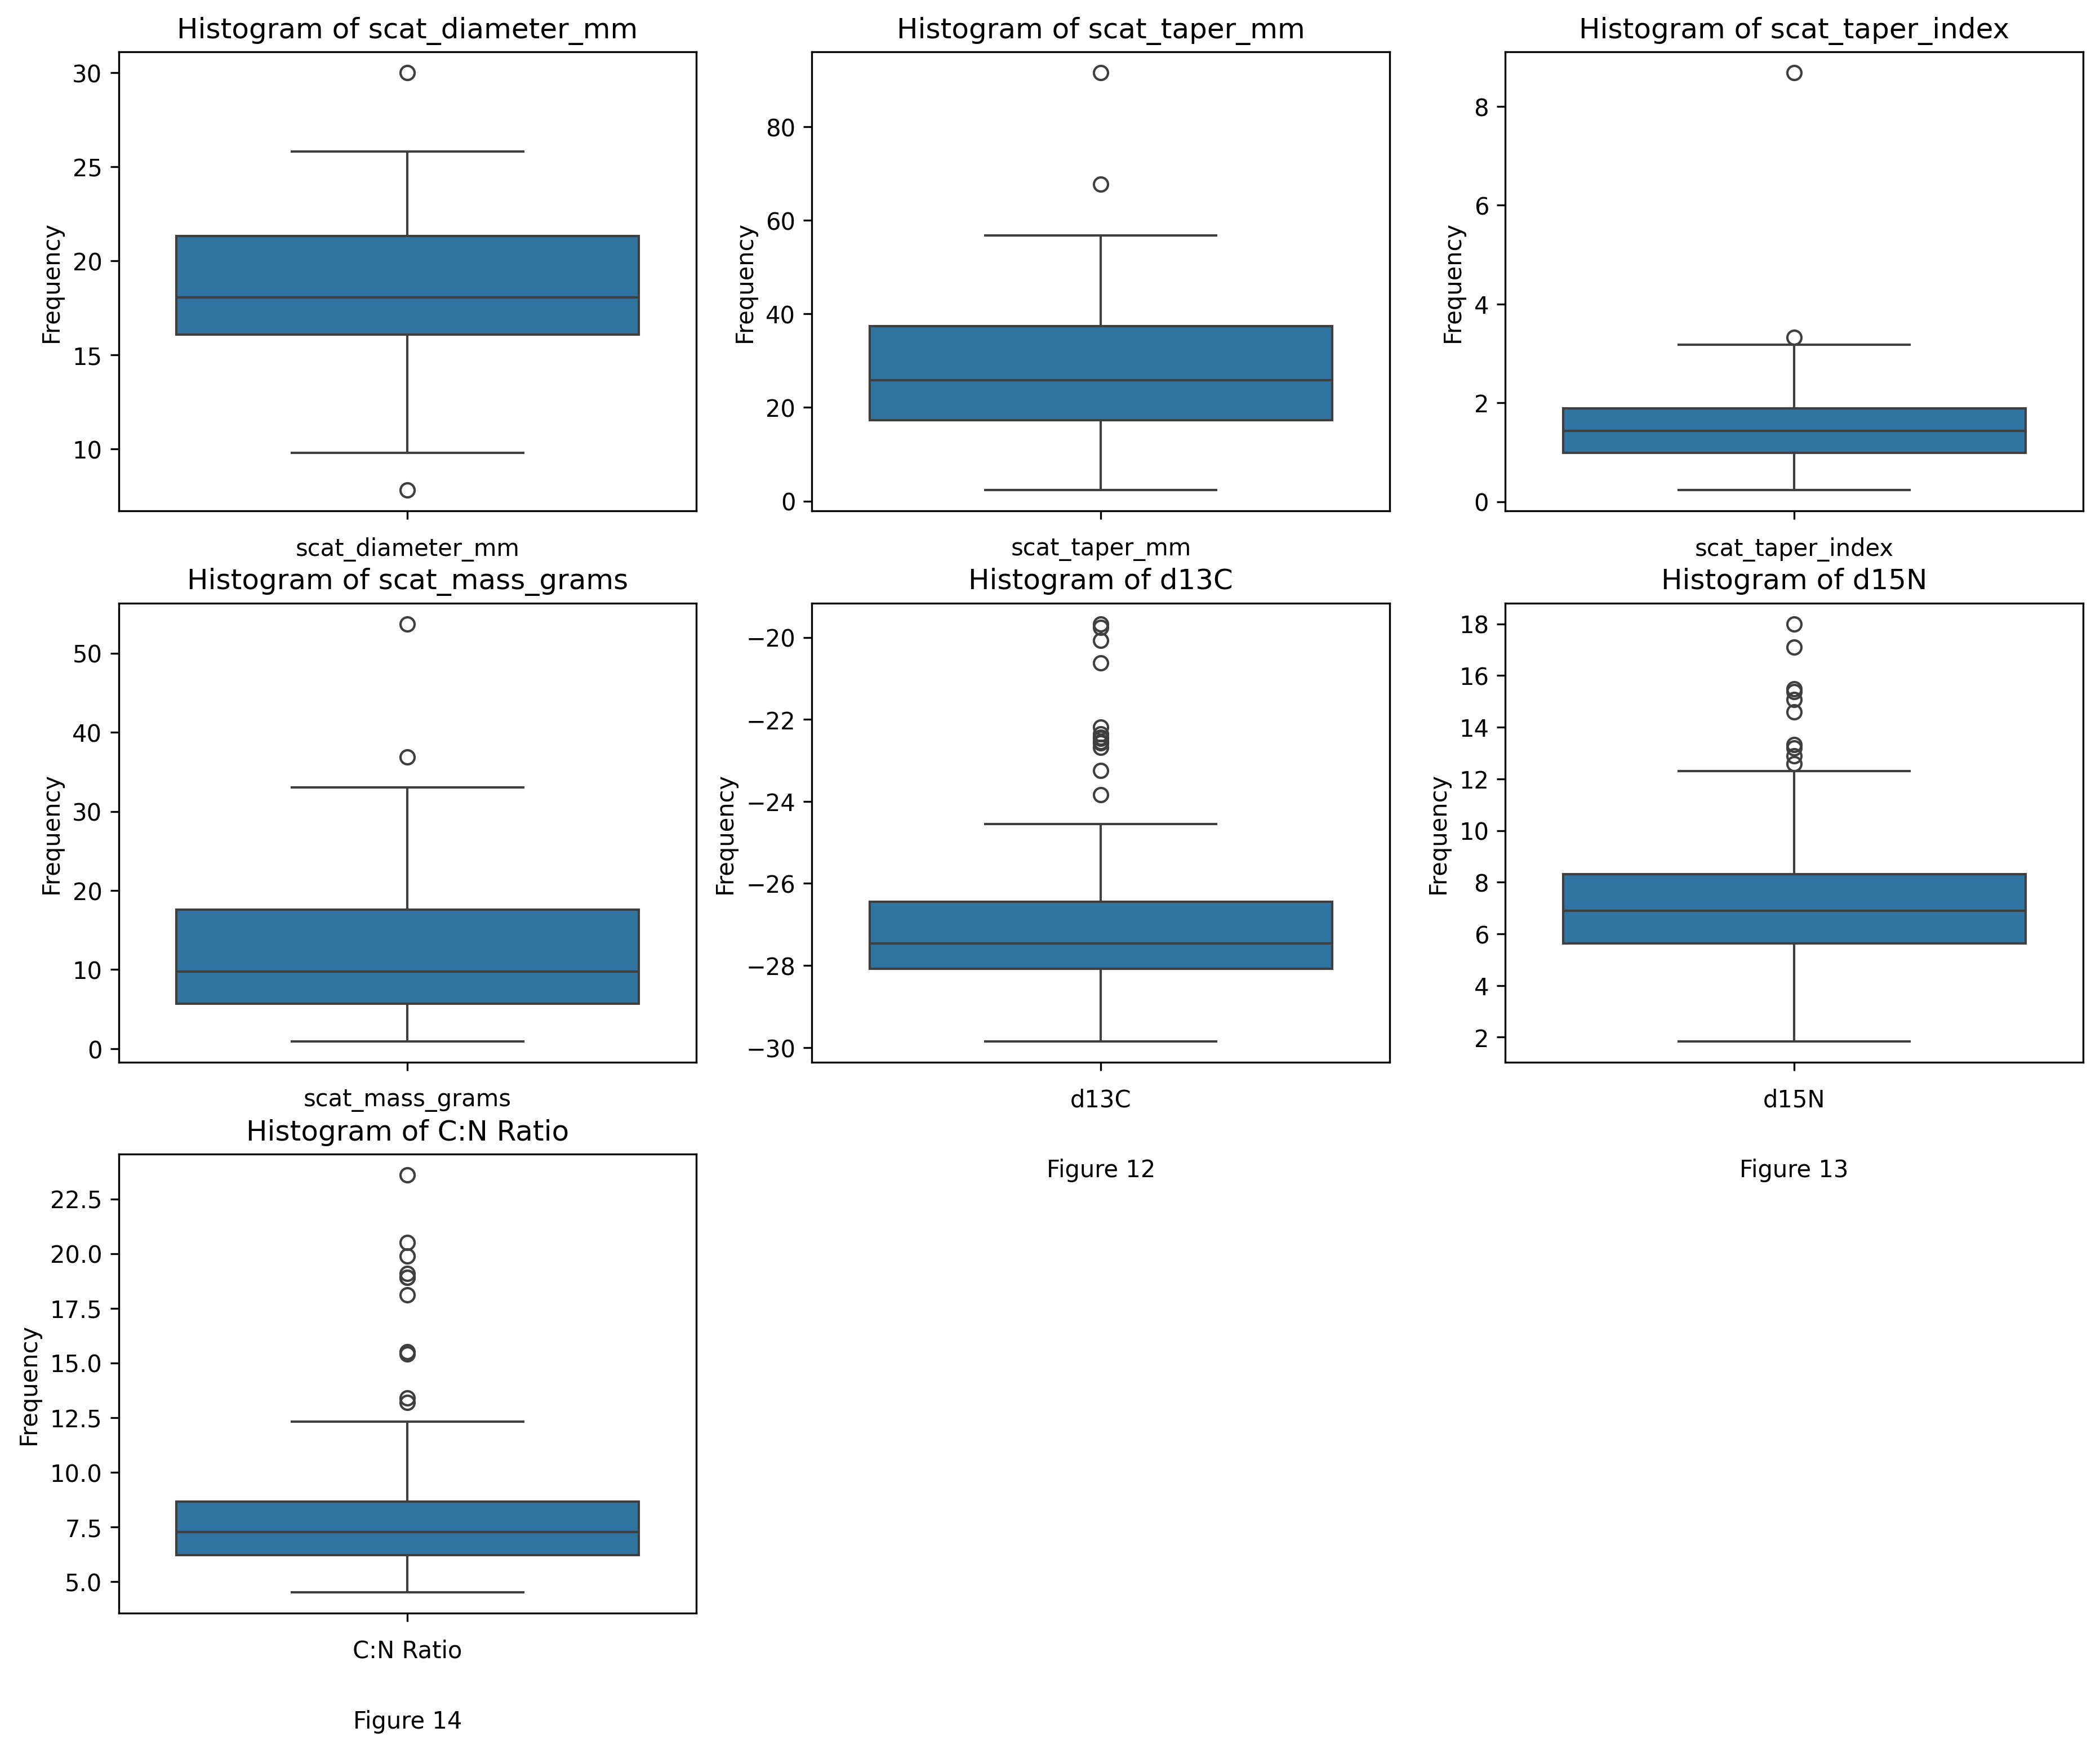
\includegraphics[width=\linewidth]{C:/GitHub/BobcatsCoyotesFoxes/plots/box_plot_missing.png}
    \end{minipage}
\end{figure}



\newpage

\subsection{The Feature Description Table}
In this section, we created a table that categorizes each variable in the data set as morphological, biogeochemical, contextual or not a trait. \\
\begin{table}[h]
    \centering
    \begin{tabular}{|c|c|c|c|} 
        \hline
        \textbf{Feature Names} & \textbf{Feature Types} & \textbf{Feature Names} & \textbf{Feature Types} \\ 
        \hline
        scat\_species & Not a Trait & scat\_age & Morphological \\ 
        \hline
        scat\_month & Contextual & scat\_number & Morphological \\ 
        \hline
        scat\_year & Contextual & scat\_length\_cm & Morphological \\ 
        \hline
        scat\_site & Contextual & scat\_diameter\_mm & Morphological \\ 
        \hline
        scat\_location & Contextual & scat\_taper\_mm & Morphological \\ 
        \hline
        scat\_taper\_index & Morphological & scat\_mass\_grams & Morphological \\ 
        \hline
        d13C & Biogeochemical & scat\_ropey & Morphological \\ 
        \hline
        d15N & Biogeochemical & scat\_segmented & Morphological \\ 
        \hline
        C:N Ratio & Biogeochemical & scat\_flat & Morphological \\ 
        \hline
        scat\_scrape & Morphological & & \\ 
        \hline
    \end{tabular}
    \caption{A Categorized Table of Features}
    \label{tab:4_columns}
\end{table}

\subsection{Imputations of Missing Value}
In this section, we look at the kernel denstiy estimation plots and the box plots to justify our reasons for the method of imputation between mean or median 
for each of the features that have missing values.

\subsubsection{Method of Imputation for \texttt{scat\_diameter\_mm}}
For this feature, if we were look at Figure 1, we can see that the histogram has a unimodal peak, and the peak is at the center of the histogram. This also
means that there is no skew at all. In Figure 8, we can see a box plot that has very few outliers and shows no skew at all too. As a result, we can say that
the feature is normally distributed, hence it should have imputations using the mode.

\subsubsection{Method of Imputation for \texttt{scat\_taper\_mm}, \texttt{scat\_taper\_index}, \texttt{scat\_mass\_grams}, \texttt{d13C}, \texttt{d15N} \& 
\texttt{C:N Ratio}}
For these following features, if we were to look at figures 2 to 7, we can see that each of them have a histrogram with a single peak, making it unimodal,
and those peaks are shifted to the left, which means that the histograms are skewed to the right.  Furthermore, when we look at the boxplots from figures
9 to 14, we can evidently see the skew, and we can also the see the huge number of outliers in figures 12 to 14. As a result, we can impute the missing values
of these features with the median.

\newpage

\subsection{Numerical Morphological Features Box Plots, Kruskal-Wallis \& Dunn Testing}
In this section, we look at all of the box plots, and we justify the use of such a visualization, as well as using Kruskal-Wallis and Dunn Testing as post-hoc.
We justify the use of box plots because we are comparing two variables which are categorical and numerical, hence a box plot  visualization would be the best.
\vspace{0.5cm}
\begin{figure}[h]
    \centering
    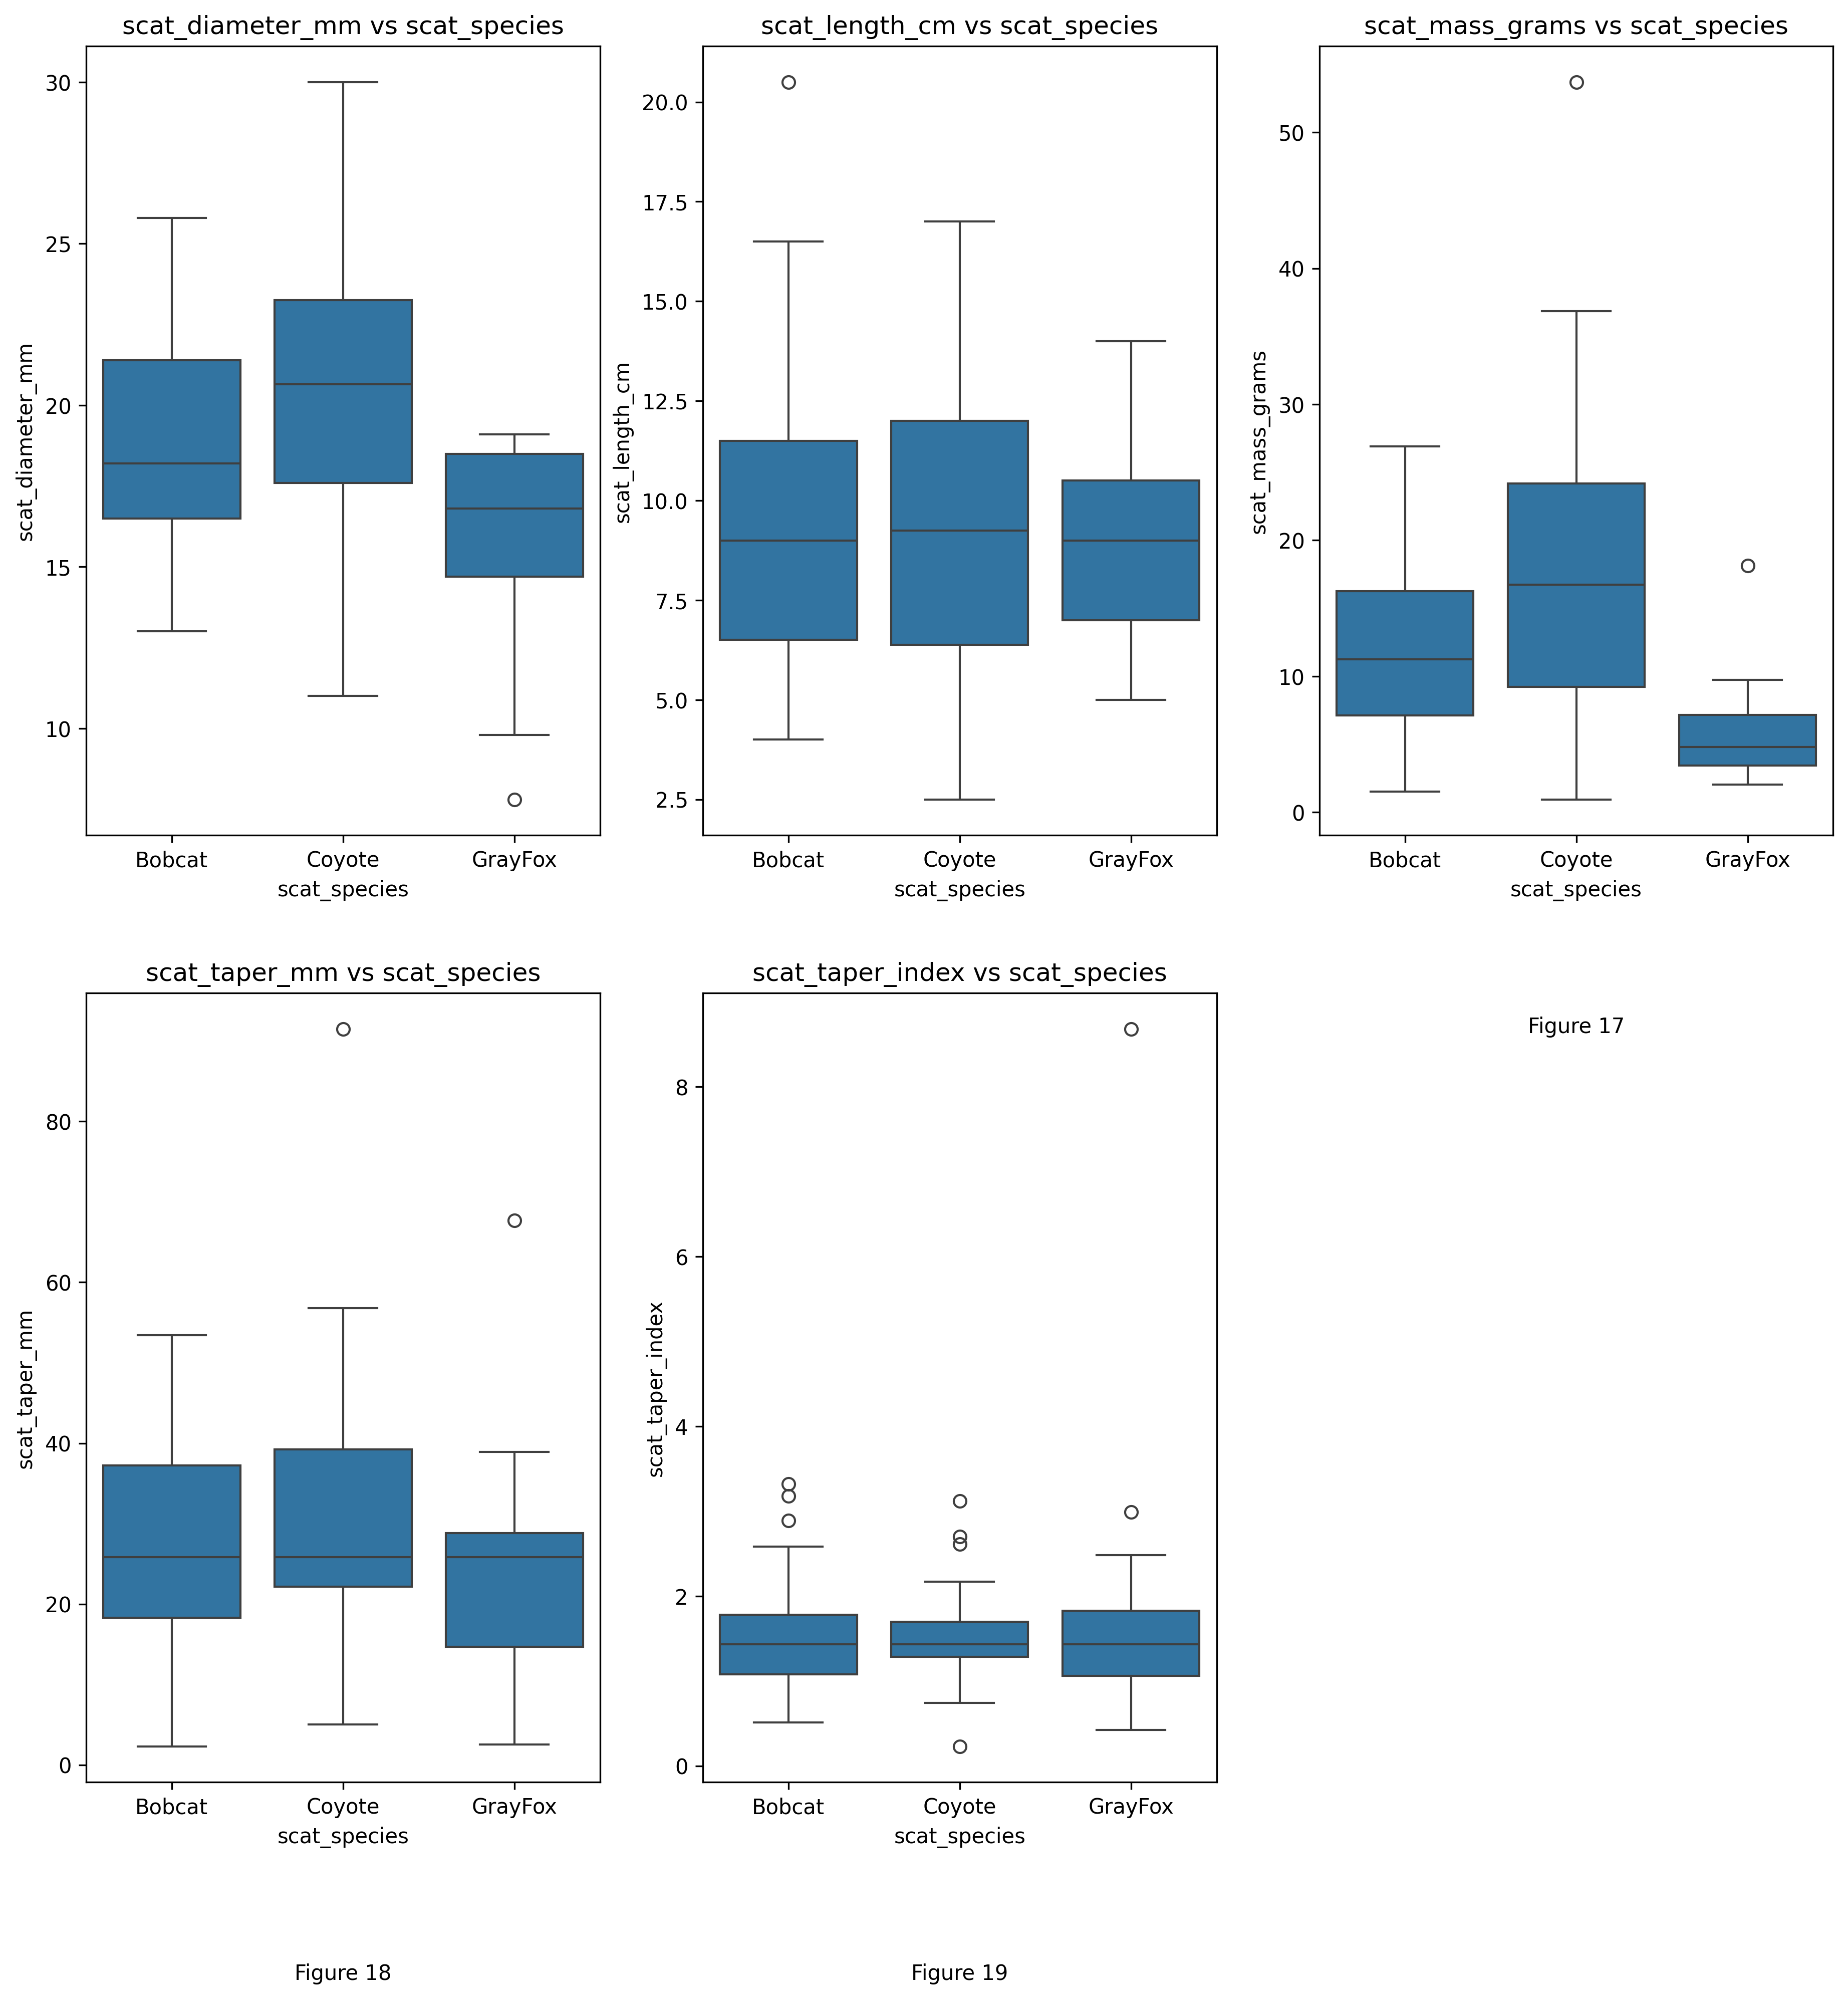
\includegraphics[width=0.8\textwidth]{C:/GitHub/BobcatsCoyotesFoxes/plots/box_plot_morphological_one.png} 
\end{figure}

\newpage

\subsubsection{\texttt{scat\_diameter\_mm} vs \texttt{scat\_species}}
When we look at figure 15, and compare the three box plots of Bobcat, Coyotes \& Foxes, we can evidently say that the medians between Gray Fox is different
compared to Bobcat \& Coyote, which suggests that the central tendency of the \texttt{scat\_diameter\_mm} is different across all three species. Furthermore, 
judging by the IQR spread of Bobcats \& Coyotes, we can say that they both have more variablility than Gray Foxes. It is worth noting that none of the 
boxplots have any outliers, which means that the data within those species is consistent. For Bobcats, we can say that the box plot has a positive skew, and 
for Coyotes, we can say that the box plot has no skew, and for Gray Foxes, the box plot has a negative skew. \\

\noindent With regards to statistical testing, it would be the most appropriate to use Kruskal-Wallis because \texttt{scat\_species} consists of three values
versus a numerical variable,which is \texttt{scat\_diameter\_mm}. After performing the Kruskal-Wallis test, we found that the test signifigance was true,
which had meant that we rejected the null hypothesis and concluded that there is a statistically significant difference between atleast one of the groups.
When performing the Kruskal-Wallis test, it is important to note that we had applied Bonferroni Correction to reduce the chances of any Type I error. \\

\noindent After performing the statistical testing, we moved on to performing a post-hoc test, where we we used Dunn's test to find out which specific 
groups are different, and the results of the test are shown below: \\
\begin{table}[h]
    \centering
    \begin{tabular}{|c|c|c|c|}
    \hline
    \textbf{Comparison} & \textbf{Bobcat} & \textbf{Coyote} & \textbf{GrayFox} \\
    \hline
    Bobcat & 1.000 & 0.208 & 0.001 \\
    Coyote & 0.208 & 1.000 & 0.000 \\
    GrayFox & 0.001 & 0.000 & 1.000 \\
    \hline
    \end{tabular}
    \caption{Dunn's Test p-values for \texttt{scat\_diameter\_mm} between Species}
    \label{tab:dunn_test_results}
\end{table}

\noindent Looking at the results of the table above, we can say that the Bobcats \& Coyotes don't show a significant different in scat diameter. Bobcats 
\& Gray Foxes show a significant difference in scat diameter and Coyotes \& Gray Foxes also show a significant difference in diamater. In conclusion, we can
say that the scat diamater of Gray Foxes is different from both Bobcats \& Coyotes, but there is no signifcant difference between Bobcats \& Coyotes. \\

\subsubsection{\texttt{scat\_length\_cm} vs \texttt{scat\_species}}
When we look at figure 16, and compare the three box plots of Bobcat, Coyotes \& Gray Foxes, we can evidently say that the medians between all three are very 
similar, which suggests that the central tendency of the \texttt{scat\_length\_cm} has little to no difference in the central values of the numerical variable
across all categories. The IQR of Gray Fox is smaller than Bobcats \& Coyotes, which suggests that Gray Foxes have less variability than the other two. It is
also worth noting that there are very few outliers in the box plots, which means that the data is consistent. It also appears that all box plots have no skew,
making them symmetrical. \\

\noindent With regards to statistical testing, it would be the most appropriate to use Kruskal-Wallis because \texttt{scat\_species} consists of three values
versus a numerical variable, which is \texttt{scat\_length\_cm}. After performing the Kruskal-Wallis test, we found that the test signfigance was false. Which
had meant that we had accepted the null hypothesis and concluded that there is no statistically significant difference between atleast one of the groups. 
When performing the Kruskal-Wallis test, it is important to note that we had applied bonferroni correction to reduce the chances of any Type I error. \\

\subsubsection{\texttt{scat\_mass\_grams} vs \texttt{scat\_species}}
When we look at figure 17, and compare the three box plots of Bobcat, Coyotes \& Gray Foxes, we can see that the medians of the box plots of Bobcat \&
Coyotes are similar, however the median of the Gray Fox is different from the rest. The IQR of the Bobcats \& Coyotes are larger than the IQR of Gray Foxes,
which means that it has more variability. All three box plots have very few outliers, which means that the data is consistent across all three. It would also
be fair to assume that there is no skew in all three box plots, as they appear to be symmetrical. \\

\noindent With regards to statistical testing, it would be the most appropriate to use Kruskal-Wallis because \texttt{scat\_species} consists of three values
versus a numerical variable, which is \texttt{scat\_mass\_grams}. After performing the Kruskal-Wallis test, we found that the signifigance test was true. 
Which had meant that we had rejected the null hypothesis and concluded that there is a statistically significant difference between atleast one of the groups.
When performing the Kruskal-Wallis test, it is important to note that we had applied Bonferroni Correction to reduce the chances of any Type I error. \\

\noindent After performing the statistical testing, we moved on to performing a post-hoc test, where we used Dunn's test to find out which specific groups are
different, and the results of the test are shown below: \\

\begin{table}[H]
    \centering
    \begin{tabular}{|c|c|c|c|}
    \hline
    \textbf{Comparison} & \textbf{Bobcat} & \textbf{Coyote} & \textbf{GrayFox} \\
    \hline
    Bobcat & 1.000 & 0.078 & 0.000 \\
    \hline
    Coyote & 0.078 & 1.000 & 0.000 \\
    \hline
    GrayFox & 0.000 & 0.000 & 1.000 \\
    \hline
    \end{tabular}
    \caption{Dunn's Test p-values for scat\_mass\_grams between species}
    \label{tab:dunn_scat_mass}
\end{table}

\noindent Looking at the results of the table above, we can say that there is no significant difference in scat mass between Bobcats \& Coyotes. We can also
say that there is a significant difference between Bobcats \& Gray Foxes, and there is a significant difference between Coyotes \& Gray Foxes. There is no
difference in scat mass between Bobcats \& Coyotes. As a result, it is the Gray Foxes that has a significant difference in scat mass with other species.

\subsubsection{\texttt{scat\_taper\_mm} vs \texttt{scat\_species}}
When we look at figure 18, and compare the three box plots of Bobcat, Coyotes \& Gray Foxes, we can see that the medians of the box plots of all three are
similar. The IQR of all three box plots are similar, which suggests that all three categories have similar variability. All three box plots also have very 
few outliers, which means that the data is consistent across all three. While the Bobcat box plot has no skew, we can deduce that the Coyote box plot has a 
positive skew, and the Gray Fox box plot has a negative skew. \\

\noindent With regards to statistical testing, it would be the most appropriate to use Kruskal-Wallis because \texttt{scat\_species} consists of three values
versus a numerical variable, which is \texttt{scat\_taper\_mm}. After performing the Kruskal-Wallis test, we found that the signifigance test was false.
Which had meant that we had accepted the null hypothesis and concluded that there no statistically signficant difference between atleast one of the groups.
When performing the Kruskal-Wallis test, it is important to note that we had applied Bonferroni Correction to reduce the chances of any Type I error. 

\subsubsection{\texttt{scat\_taper\_index} vs \texttt{scat\_species}}
When we look at figure 19, and compare the three box plots of Bobcat, Coyotes \& Gray Foxes, we can see that the medians of the box plots of all three are
similar. The IQR of all three box plots are similar, although the IQR of the Coyote box plots seems a little  smaller, however, this overall indicates that
all three categories have similar variability. All three box plots have few outliers, which means that the data is consistent across all three categories.
It can also be seen that alll three box plots have no skew. \\

\noindent With regards to statistical testing, it would be the most appropriate to use Kruskal-Wallis because \texttt{scat\_species} consists of three values
versus a numerical variable, which is \texttt{scat\_taper\_index}.  After performing the Kruskal-Wallis test, we found that the signifigance test was false.
Which had meant that we had accepted the null hypothesis and concluded that there no statistically signficant difference between atleast one of the groups.
When performing the Kruskal-Wallis test, it is important to note that we had applied Bonferroni Correction to reduce the chances of any Type I error. \\

\newpage

\subsection{Numerical Biogeochemical Features Box Plots, Kruskal-Wallis \& Dunn Testing}
In this section, we look at all of the violin plots, and we justify the use of such a visualization, as well as using Kruskal-Wallis and Dunn Testing as 
post-hoc. We justify the use of violin plots because we are comparing two variables which are categorical and numerical, hence a violin plot visualization 
would be the best.
\vspace{0.5cm}
\begin{figure}[h]
    \centering
    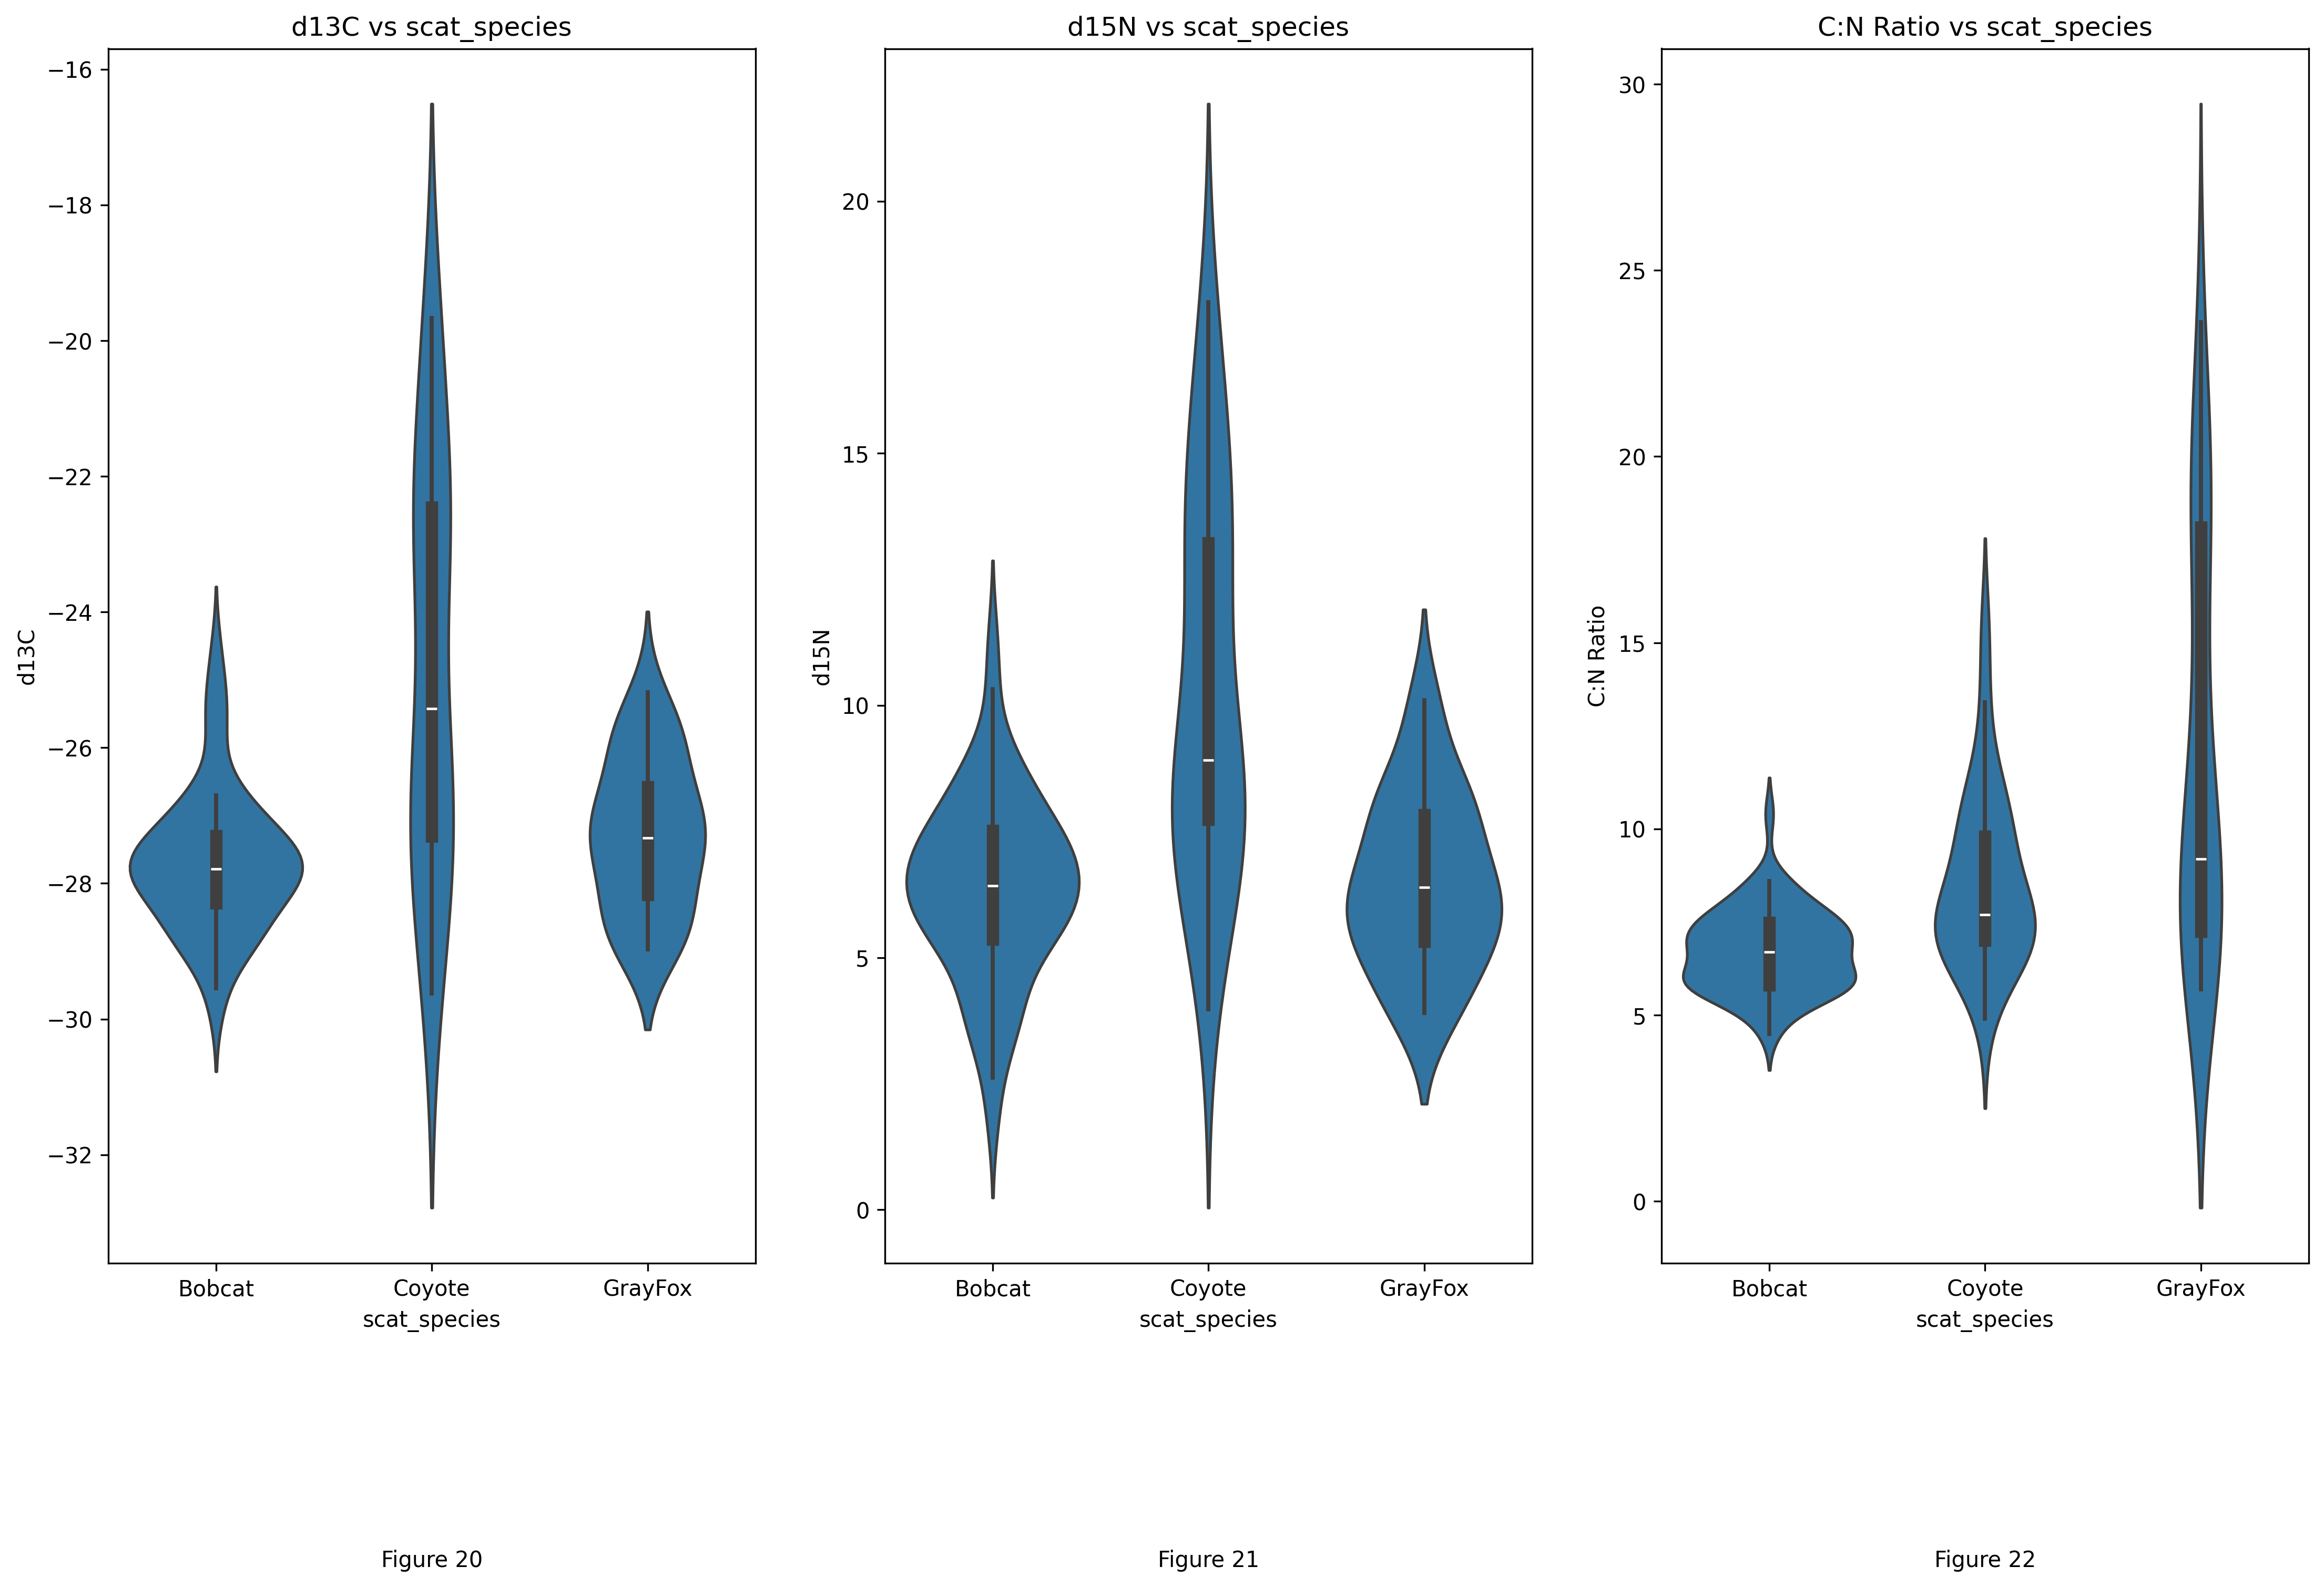
\includegraphics[width=0.8\textwidth]{C:/GitHub/BobcatsCoyotesFoxes/plots/violin_plot_biogeochemical.png} 
\end{figure}



\subsubsection{\texttt{d13C} vs \texttt{scat\_species}}
When we look at figure 24, and compare the three violin plots of Bobcat, Coyotes \& Gray Goxes, the medians of the Gray Foxes and Bobcats are similar, however
the median of the Coyote violin plot is very different from the rest. When it comes to comparing the IQR of all three violin plots, we can deduct that the
Coyote violin plot has the most spread, compared the IQR of both Bobcat \& Gray Fox, which appear to be similar. It can be seen that the violin plot of 
Bobcat, has a left skew, the Coyote violin plot has no skew, and the Gray Fox violin plot has no skew either. \\

\noindent With regards to statistical testing, it would be the most appropriate to use Kruskal-Wallis because \texttt{scat\_species} consists of three values
versus a numerical variable, which \texttt{d13C}. After performing the Kruskal-Wallis test, we found that the signifigance test as true. Which has meant that
we have rejected the null hypothesis and concluded that there is a statistically signifcant difference between atleast one of the groups. When performing the
Kruskal-Wallis tests, it is important to note that we had applied the Bonferroni Correction to reduce the chances of any Type I error. \\

\noindent After performing the statistical testing, we moved on to performing a post-hoc test, where we used Dunn's test to find out which specific groups are
different, and the results of the test are shown below: \\

\begin{table}[h!]
    \centering
    \begin{tabular}{|c|c|c|c|}
    \hline
    \textbf{Comparison} & \textbf{Bobcat} & \textbf{Coyote} & \textbf{GrayFox} \\
    \hline
    Bobcat & 1.000 & 0.000 & 0.160 \\
    \hline
    Coyote & 0.000 & 1.000 & 0.010 \\
    \hline
    GrayFox & 0.160 & 0.010 & 1.000 \\
    \hline
    \end{tabular}
    \caption{Dunn's Test p-values for d13C between species}
    \label{tab:dunn_d13C}
\end{table}




\end{document}

